\normaltrue \difficilefalse \tdifficilefalse
\correctionfalse
%\UPSTIidClasse{11} % 11 sup, 12 spé
%\newcommand{\UPSTIidClasse}{11}

\exer{ $\star$ \label{B2:16:64}}
%% CCP MP 2007
\setcounter{numques}{0}
\UPSTIcompetence[2]{B2-16}
\index{Compétence B2-16}

\index{EPAS}
\index{Hyperstatisme}

\ifcorrection
\else
\textbf{Pas de corrigé pour cet exercice.}
\fi

\ifprof
\else
On s'intéresse à l'échelle pivotante équipant un camion de pompier.


\begin{center}
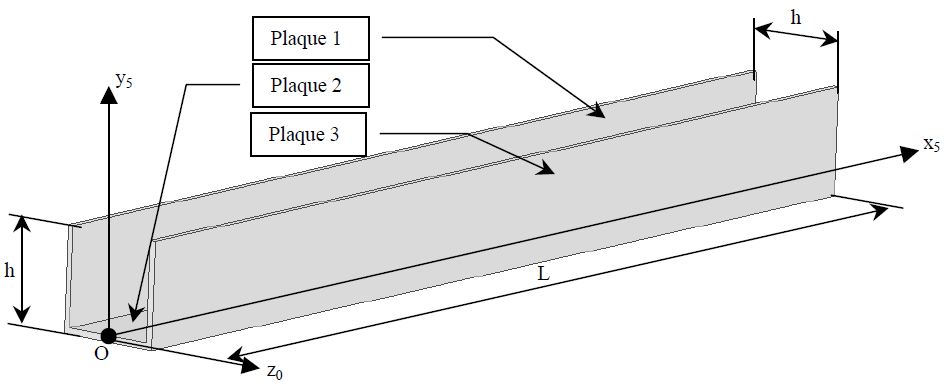
\includegraphics[width=\linewidth]{64_01}
\end{center}

On donne un schéma cinématique du système de manoeuvre du parc échelle.

\begin{center}
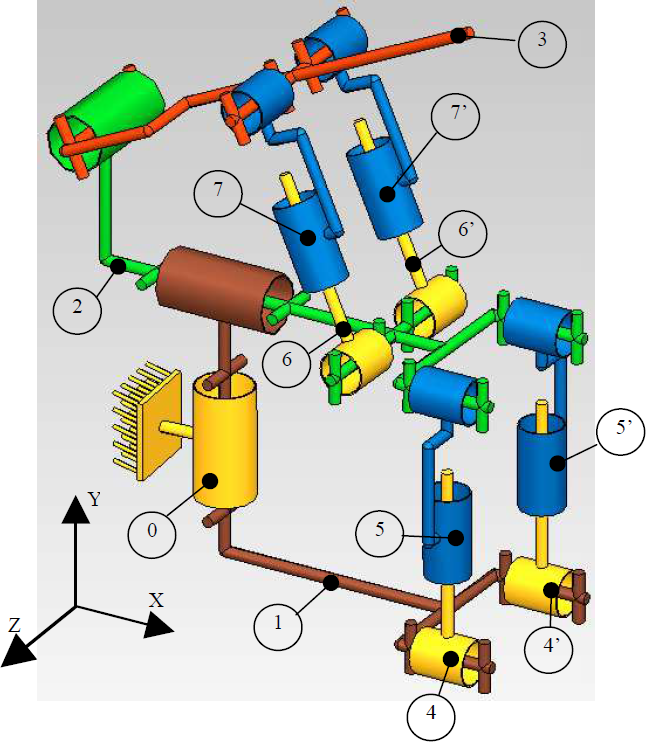
\includegraphics[width=\linewidth]{64_02}
\end{center}

\fi

\question{Réaliser le graphe des liaisons.}
\ifprof
\else 
\fi

\question{Déterminer le degré d’hyperstatisme de ce mécanisme.}
\ifprof
\else 
\fi

\question{Proposer des modifications qui permettraient de le rendre isostatique.}
\ifprof
\else 
\fi
 
 

\ifprof
\else

\noindent\footnotesize
 \fbox{\parbox{.9\linewidth}{
 Éléments de corrigé : 
 \begin{enumerate}
\item .
\item $h=8$.
\item .
 \end{enumerate}}}
\normalsize

\begin{flushright}
\footnotesize{Corrigé  voir \ref{B2:16:64}.}
\end{flushright}%
\fi